\documentclass[final]{beamer}
\usepackage[ngerman]{babel}
\usepackage[utf8]{inputenc}
\usepackage[T1]{fontenc}
\usepackage{lmodern}
\usepackage{listings}
\usepackage{graphicx}
\usepackage{color}
\usepackage{amssymb}
\newcommand{\ThemeFolder}{./FSIBeamerTheme}
\RequirePackage{\ThemeFolder/beamerthemeFSI}

\DeclareGraphicsExtensions{.pdf,.png}

\mode<presentation>


\title{Programmiervorkurs für Erstsemester}

\setbeamertemplate{title page}{
  \begin{center}
	{\usebeamerfont{title}\usebeamercolor[fg]{title}\inserttitle}
  \end{center}
  
}

\begin{document}
\shorthandoff{"}
\lstset{tabsize=2}
\lstset{basicstyle=\small}
\lstset{language=java}
\lstset{showstringspaces=false}
\begin{frame}
  \titlepage
\end{frame}

\section{Über mich}
\begin{frame}
	\frametitle{Über mich}
	\textbf{Moritz Grimm}
	\begin{itemize}
		\item{5. Semester Informatik}
		\item{aktiver Fachschafter}
		\item{Kassenwart des Fachschaftsvereins}
	\end{itemize}
\end{frame}

\section{Inhalte}
\begin{frame}
	\frametitle{Inhaltsübersicht Vorkurs}
	\begin{itemize}
		\item {Tag 1: Variablen, Datentypen, Konvertierungen, Arithmetik, Netbeans, Einführung Debugging}
		\item {Tag 2: Boolesche Ausdrücke, Kommentare, If-Abfragen, Switch-Case, Weiterführung Debugging}
		\item {Tag 3: Arrays, (Do-)While-Schleife, For-Schleifen, Weiterführung Debugging}
		\item {Tag 4: (statische) Methoden, Attribute, Ausführung Debugging}
	\end{itemize}
\end{frame}

\begin{frame}
	\frametitle{Inhaltsübersicht Tag 2}
	\begin{itemize}
		\item {Boolesche Ausdrücke}
		\item {Kommentare}
		\item {If-Abfragen}
		\item {Switch-Case}
		\item {Weiterführung Debugging}
	\end{itemize}
\end{frame}

\section{Kommentare}
\begin{frame}
	\frametitle{Kommentare}
	\begin{itemize}
		\item{Erleichtern das Verständnis des Quelltextes}
		\item{haben keinen Einfluss auf den Programmablauf}
		\item{Programmdokumentation durch Javadoc}
	\end{itemize}
\end{frame}

\subsection{Arten}
\begin{frame}[containsverbatim]
	\begin{lstlisting}
Javadoc:
/**
* Kommentar (auch ueber mehrere Zeilen), der
* automatisch zu html-Dokumentation
* verarbeitet werden kann
*/
Blockkommentar:
/*
* Mehrzeilige Kommentare sind ideal, wenn
* viele Informationen unterzubringen sind.
* Es gilt die Devise: so knapp wie
* moeglich, so ausfuehrlich wie noetig.
*/
Zeilenkommentar:
// endet mit Zeilenumbruch
	\end{lstlisting}
\end{frame}

\subsection{Verwendung}
\begin{frame}
	\frametitle{Verwendung von Kommentaren}
	\begin{itemize}
		\item{Nachfolgenden Entwicklern Hinweise geben, wie der Quelltext zu verstehen ist}
		\item{Sehr praktisch als Gedächtnisstütze: TODOs setzen}
		\item{Zum Testen können Teile des Quellcodes zeitweise auskommentiert werden}
		\item{Javadoc und Blockkommentare stehen über der zu kommentierenden Klasse oder Methode}
	\end{itemize}
\end{frame}

\subsection{Beispiel}
\begin{frame}[containsverbatim]
\frametitle{Beispiel}
	\begin{lstlisting}
/**
* This Class is dangerous! Do not execute it.
* @author memo
*/
public class GladOS {
	/*
	* Die wichtigste Methode: 
	* alles was ausgefuehrt wird muss zumindest 
	* hier aufgerufen werden.
	*/
	public static void main(String[] args){
		// the cake is a lie
		boolean cake = true;
	}
}

	\end{lstlisting}
\end{frame}

\begin{frame}
	\frametitle{Deklaration einer Methode mit Javadoc.}
	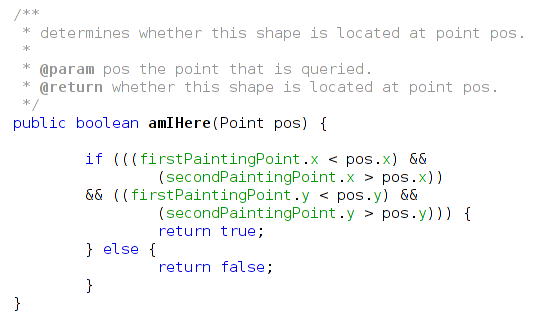
\includegraphics[scale=0.5]{JavaDoc_example_1_1.png}
\end{frame}

\begin{frame}
	\frametitle{Verwendung der Methode mit Javadoc.}
	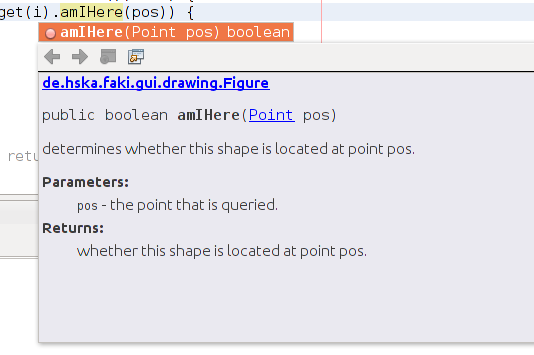
\includegraphics[scale=0.5]{JavaDoc_example_2_1.png}
\end{frame}

\section{boolean}
\subsection{Wahrheitswerte}
\begin{frame}
	\frametitle{Boolsche Ausdrücke - Wahrheitswerte}
	\textbf{100 Fakten zu Boolschen Ausdrücken}
	\begin{itemize}
		\item{entweder wahr oder falsch}
		\item{oft das Ergebnis eines Vergleichs}
		\item{können kombiniert werden}
		\item{werden zur Entscheidungsfindung verwendet}
	\end{itemize}
\end{frame}


\subsection{Vergleiche}
\begin{frame}
	\frametitle{Boolsche Operatoren - Vergleiche}
	\begin{itemize}
		\item{>  - größer}
		\item{<  - kleiner}
		\item{>= - größer gleich}
		\item{<= - kleiner gleich}
		\item{== - gleich}
		\item{!= - ungleich}
	\end{itemize}
\end{frame}

\subsection{Verknüpfungen}
\begin{frame}
	\frametitle{Boolsche Operatoren - Verknüpfungen}
	\begin{tabular}{c c c}
		\textbf{\&}  & - & und \\&&\\
		\textbf{|} & - & oder \\&&\\
		\textbf{!} & - & nicht \\&&\\
		\textbf{\^\ }  & - &  exlusives oder \\&&\\
		\textbf{==} & - & gleich \\&&\\
		\textbf{!=} & - & ungleich \\
	\end{tabular}
	\
\end{frame}

\begin{frame}
	\frametitle{Wahrheitstabellen}
	\center{0 - false, 1 - true} \\
	\begin{center}
	\begin{tabular}{c  c c}
		\begin{tabular}{c c c c c | c}
			& \textbf{a}  & & \textbf{b} & & \textbf{\&} \\
			\hline
			& 0 & & 0 & &  0\\
			& 0 & & 1 & &  0\\
			& 1 & & 0 & &  0\\
			& 1 & & 1 & &  1\\
		\end{tabular}
		& &
		\begin{tabular}{c c c c c | c}
			& \textbf{a}  & & \textbf{b} & & \textbf{|} \\
			\hline
			& 0 & & 0 & &  0\\
			& 0 & & 1 & &  1\\
			& 1 & & 0 & &  1\\
			& 1 & & 1 & &  1\\
		\end{tabular}
		\\ &\\ &\\
	\begin{tabular}{c c c c c | c}
			& \textbf{a}  & & \textbf{b} & & \textbf{\^} \\
			\hline
			& 0 & & 0 & &  0\\
			& 0 & & 1 & &  1\\
			& 1 & & 0 & &  1\\
			& 1 & & 1 & & 0\\
	\end{tabular}
	& &
\begin{tabular}{c c c | c}
		& \textbf{a} & & \textbf{!} \\
		\hline
		& 0 & & 1\\
		& 1 & & 0\\
	\end{tabular}
	\\
	\end{tabular}
	\end{center}
\end{frame}

\subsection{Operatoren}
\begin{frame}
	\frametitle{Kurzschlussoperatoren}
	\begin{itemize}
		\item{UND und ODER gibt es auch als sogenannte Kurzschlussoperatoren: \&\& und ||}
		\item{=> Der Ausdruck wird nur solange ausgewertet, bis das Ergebnis feststeht}
	\end{itemize}
\end{frame}

\begin{frame}
	\frametitle{Rangfolge der Operatoren}
	\center{Sortiert nach absteigender Bindungsstärke}\\
	\begin{center}
	\begin{tabular}{|l c | l|}
	 \hline
		++, -- --  & &  Inkrement und Dekrement \\
		 \hline
		! & & Negation \\ \hline
		
		*, /, \% & & Multiplikation, Division, Modulo \\ \hline
		+, - & & Addition und Subtraktion \\ \hline
		==, != & & Vergleich \\ \hline
		\& & & Und \\ \hline
		| & & Oder \\ \hline
		\&\& & & Kurzschlussoperator Und \\ \hline
		|| & & Kurzschlussoperator Oder \\ \hline
		= & & Zuweisung \\
		 \hline
	\end{tabular}
	\center{Unäre Operatoren => Standard Rechenzeichen => binäre Operatoren => Zuweisungen}
	\end{center}
\end{frame}

\subsection{boolscher Ausdruck} 
\begin{frame}
	\frametitle{Definition: boolscher Ausdruck}
	\begin{itemize}
		\item{Bedingung A - kann wahr oder falsch sein}
		\item{(Bedingung A || Bedingung B) \&\& Bedingung C}
		\item{"Ich habe den Compagnion Cube" \&\& "Ich bin unsterblich" (kann der Compiler so nicht auswerten, Menschen schon)}
	\end{itemize}
\end{frame}

\subsection{Beispiel}
\begin{frame}
	\frametitle{Beispiel: \\Schreibe einen boolschen Ausdruck in Java Syntax, der einen Sportwagen erkennt}
	Unsere Definition eines Sportwagens:	\\
	\begin{itemize}
		\item{maximal zwei Türen, keine Rücksitze, außerdem:}
		\item{Höchstgeschwindigkeit von mindestens 200 km/h und  Mindestbeschleunigung von 0 auf 100 km/h in 8 Sekunden}
		\item{oder Höchstgeschwindigkeit von mindestens 280 km/h und mindestens 250 PS}
	\end{itemize}
\end{frame}

\begin{frame}[containsverbatim]
	\frametitle{Auszuwertende Variablen}
	\begin{lstlisting}
boolean hatRuecksitze; 
// dann true, wenn das Auto Ruecksitze hat
int tueren; // Anzahl Tueren
double beschleunigung; 
// in Sekunden von 0 auf 100
double hoechstgeschwindigkeit; // in km/h
double leistung; // in kW (nicht in PS!)
1 PS ~ 0,735 kW
	\end{lstlisting}
\end{frame}

\section{Gleitkommazahlen}
\begin{frame}
	\frametitle{Exkurs: Gleitkommazahlen}
	\begin{itemize}
		\item{Gleitkommazahlen in Java sind anfällig für Rundungsfehler}
		\item{Zahlen die im Dezimalsystem endlich sind, sind das nicht zwangsläufig auch im Binärsystem}
		\item{z.B. 0,1 Dezimal == 0,00011001100110011... Binär}
		\item{=> 1.0 - (0.1 + 0.1 + 0.1 + 0.1 + 0.1 + 0.1 + 0.1 + 0.1 + 0.1 + 0.1) != 0.0}
	\end{itemize}
\end{frame}

\subsection{Vergleiche}
\begin{frame}
	\frametitle{Exkurs: Gleitkommazahlen}
	\begin{itemize}
		\item{Schon der Variablentyp kann einen Unterschied machen}
		\item{0.02d (double) == 0.02f (float) ?}
		\item{=> Um sicherzugehen lieber prüfen, ob die Abweichung nur minimal ist: \\ 
		Math.abs(0.02d - 0.02f) < 4.5E-10 ?}
		\item{Math.abs(zahl) berechnet den Betrag von zahl}
	\end{itemize}
\end{frame}

\subsection{Größenordungsprobleme}
\begin{frame}
	\begin{itemize}
		\item{Achtung beim Verrechnen von Zahlen die einige Größenordungen auseinander liegen}
		\item{z.B. 100000000000000000.0 + 8 = 100000000000000000.0}
		\item{Grund: Gleitkommazahlen werden als Basis und Exponent gespeichert}
		\item{Die Basis muss alle relevanten Teile der Zahl enthalten die dann vom Exponent verschoben werden können}
		\item{=> Es können sehr große und sehr kleine Zahlen gespeichert werden, aber nicht beides}
	\end{itemize}
\end{frame}

\section{if}
\subsection{Beispiel}
\begin{frame}[containsverbatim]
	\frametitle{Fallunterscheidung durch if-Abfragen}
	Anweisung wird nur dann ausgeführt, wenn eine bestimmte Bedingung erfüllt ist:
	\begin{lstlisting}
if (Bedingung) {
	// mach was
} else if (andere Bedingung){
	// mach was anderes
} else {
	// lass es bleiben
}
	\end{lstlisting}
	(else if und else optional)
\end{frame}

\begin{frame}[containsverbatim]
	\frametitle{}
	\begin{lstlisting}
String answer = "studying";
if (answer == "Cake") {
	System.out.println("nice try");
} else if (answer == "42"){
	System.out.println("You got it!");
} else if (answer == "studying"){
	System.out.println("Not to everything,
                       but very commendable");
} else {
	System.out.println("think harder!")
}
	\end{lstlisting}
\end{frame}

\subsection{Syntax}
\begin{frame}
	\frametitle{if-Abfragen - Syntax}
	\begin{itemize}
		\item{Auf die Klammer, in der die Bedingung angegeben wird, folgt kein Semikolon!}
		\item{In einem If-Block können beliebig viele Anweisungen stehen.}
		\item{Die einzelnen Blöcke werden durch geschweifte Klammern getrennt}
	\end{itemize}
\end{frame}

\begin{frame}[containsverbatim]
	\frametitle{noch ein etwas praktischeres Beispiel:}
	\begin{lstlisting}
double a, b;
...
if (a != 0.0) {
	System.out.print("b/a: ");
	System.out.println(b/a);
} else {
	System.out.println("Division durch 0!");
}
	\end{lstlisting}	
	Hier ist die Bedingung das Ergebnis eines Vergleichs.	
\end{frame}

\subsection{false == true}
\begin{frame}[containsverbatim]
	\frametitle{Abkürzungen bei boolschen Variablen}
	\begin{lstlisting}
boolean istStudent = true;
if (!istStudent) {
	// gewaehre keinen Studentenrabatt
}
entspricht der Abfrage folgender Bedingungen:
if (istStudent == false) { ... }
if (!(istStudent == true)) { ... }

	\end{lstlisting}
\end{frame}

\subsection{Verschachtelung}
\begin{frame}[containsverbatim]
	\frametitle{Verschachtelte if-Abfragen}
	\begin{lstlisting}
long losnummer;
...
if (losnummer > 3) {
	if (losnummer % 315 == 4) {
		System.out.println("Gewinnerlos");
	}
} else {
	System.out.println("Verliererlos");
}
	\end{lstlisting}
	=> Vorsicht! Wird leicht unübersichtlich!
\end{frame}

\section{switch-case}
\subsection{Überblick}
\begin{frame}[containsverbatim]
	\frametitle{Fallunterscheidung durch Switch/Case}
	\begin{itemize}
		\item{Fallunterscheidung in Abhängigkeit von einer Variablen}
		\item{nur ganzzahlige Typen oder char}
		\item{Anweisungen für alle relevanten Werte, die die Variable annehmen kann}
	\end{itemize}
\end{frame}

\subsection{Details}
\begin{frame}[containsverbatim]
  \frametitle{Fallunterscheidung durch Switch/Case}
  \begin{itemize}
	\item{jeder Wert darf nur einmal vorkommen}
	\item{läuft durch bis break oder bis zum Ende des Switch}
	\item{trifft keiner der beachteten Fälle ein wird (ähnlich dem else) ein default ausgeführt}
  \end{itemize}
\end{frame}


\subsection{Beispiele}
\begin{frame}[containsverbatim]
	\frametitle{Beispiel}
	\begin{lstlisting}
int fall;
...
switch (fall) {
case 0:
	System.out.println("Operation erfolgreich");
	break;
case 1:
	System.out.println("Abgebrochen");
	// fall through
case 2:
	System.out.println("Operation gescheitert");
	break;
default:
	System.out.println("Unbekannter Fall!");
}
	\end{lstlisting}
\end{frame}

\begin{frame}[containsverbatim]
\frametitle{switch/case verglichen mit if/else}
	\begin{tabular}{c c c c}
	\begin{lstlisting}
char a;
...
switch (a) {
case 'r':
	// lese Eingabe
	break;
case 'q':
	// beenden
	break;
case 'n':
	// Neustart
	break;
}
	\end{lstlisting} 

& & &
	
	\begin{lstlisting}
char a;
...
if (a == 'r') {
	// lese Eingabe
} else if (a == 'q') {
	// beenden
} else if (a == 'n') {
	// Neustart
}
	\end{lstlisting}\\
	\end{tabular}
\end{frame}

\section{weitere Planung}
\begin{frame}
\frametitle{weitere Planung}
  \begin{itemize}
	\item{weiter gehts in ca. 90min}
	\item{heute Nachmittag bleiben wir da bis ihr fertig seid, es gibt also kein festes Ende bis zu dem ihr fertig sein müsst}
	\item{morgen früh ab 9:30 Uhr findet die Besprechung der Aufgaben von heute Nachmittag statt}
	\item{danach (ca. ab 10:00 Uhr) beginnt die nächste Vorlesung. Themen: Arrays und Schleifen}
	\item{außerdem bin ich der Meinung, dass englische Inhalte nicht übersetzt werden sollten.}
  \end{itemize}
\end{frame}

\end{document}
